\documentclass{llncs}
\usepackage{subcaption}
\usepackage{subfig} 
\usepackage{usual}
\usepackage{graphicx}
\usepackage[rflt]{floatflt}
%\pagestyle{plain}
%
\begin{document}
\title{\vskip -10pt Report on the implementation of the ToM}

\maketitle 

\section{Decisional function}

The first step of our implementation was to enable the negotiator agent to express strategies of negotiations relative to its power. The second step is to allow the agent to adapt its strategy of negotiation to its partner. Therefore, the agent must have a mental representation of its partner's power. We aim to use the ToM representation in order to implement this mental model. More precisely, we will use a reflexive representation of the ToM, which means that the agent will use its model model of negotiation and decision in order to reflect a model of decision of its partner.  
 
 %The agent has to 'guess' the other representation of power from the available knowledge gathered from the dialogue (enunciated utterances).
 
Thus, we have to analyze the functions that the agent uses to take a decision (\emph{i.e} choose an utterance). Based on our model of the dialogue, the choice of the next utterance to enunciate is computed with a function called 
$computeUtt$ $(Model, u^{-1}, pow) \rightarrow u$ that takes as input the following information:
\begin{enumerate}
	\item $model$: Agent's mental state in terms of the agent preferences and the current context of the dialogue (proposals, statements ...).
	
	\item $u^{-1}$ the previous utterance enunciated by the other agent.
	
	\item $pow$ the relation of power of the agent. 

\end{enumerate}
The output of this function is the utterance that the agent will enunciate in its negotiation turn.


In order to 'guess' the other representation of power from the available knowledge gathered from the dialogue (enunciated utterances). We propose to add to the agent mental state, a set of hypotheses on the possible mental state of other agent. $H_m= \{<Model_1, Pow1>, \ldots, <Model_n, pow_n> \}$. After each negotiation turn, when other enunciates an utterance, we call the decisional function on all the elements of $H_m$ and we only keep the models that produced the same utterance enunciated by the other agent.
This operation is repeated after each dialogue turn until all the remained elements in $H_m$ are defined with the same values of power $pow_1 = pow_2 = \ldots = pow_n$.

I decomposed the implementation of the ToM in several steps. 

	\subsubsection{Step 1:} We assume that the agent knows the model of preferences of the other agent. thus we make hypotheses only on the other value of power. 
	$H_m= \{<Model, Pow1>, <Model, Pow2>\ldots, <Model, pow_n> \}$.

	We call after each turn $computeUtt$ on each model of $H_m$. An example of execution is given in \fig{ex}. Agent 1 is initiated with $pow =0.9$ and Agent 2 is initiated with $pow =0.4$. Agent1 is implemented with the function to guess the power of Agent 2 after each turn of Agent2.

	We can observe that after the first utterance, the algorithm is able to guess that Agent 2 is in the submissive range of power. However, at the end, two values are kept $0.4,0.5$ because they generate the same utterances.
	
	 \begin{figure} [h]
	 	\centerline{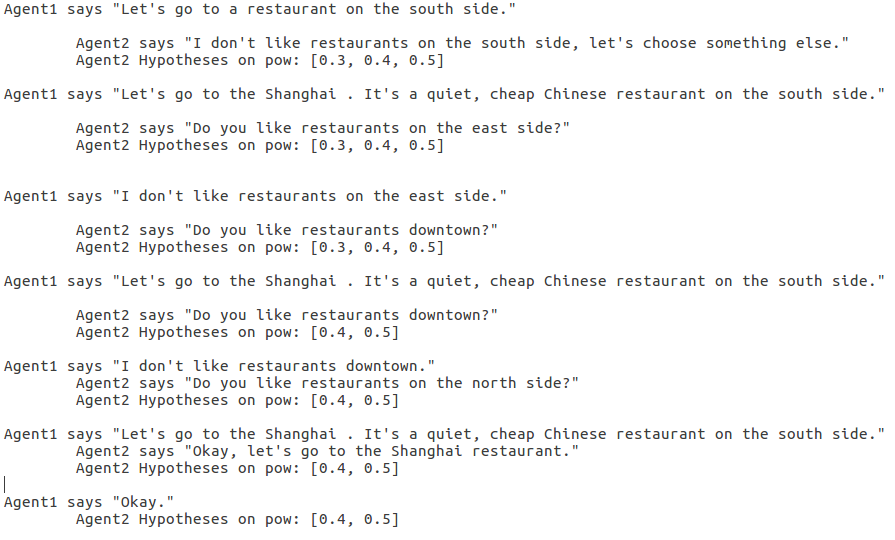
\includegraphics[width=5in]{figs/ex.png}}
	 	\vskip 8pt
	 	\defig{ex}{Example of dialogue between Agent 1 with pow =0.9 and Agent 2 with pow=0.4}
	 \end{figure}
	 
	
	\subsubsection{Step 2:} Once the function was tested and the agent was able to guess the power of other. I wrote the code to generate all the possible model of preferences for a given topic of negotiation. An agent has a set of preferences for each criterion. The combination of all possible preferences is of the order of $\prod_{c\in\mathcal{C}} |c|!$. 
	
	In addition, we have to take into account the combination of all the preferences for each criterion to create all the possible preferences models.
	In order to prevent a combinatory explosion due to the large set of all the possible preferences,I've made a test of complexity of the function $computeUtt$ on one model. The results are presented in \fig{compl} where the horizontal axis represents the number of execution o$computeUtt$ and y-axis represents the time execution. 

		 \begin{figure} [t]
		 	\centerline{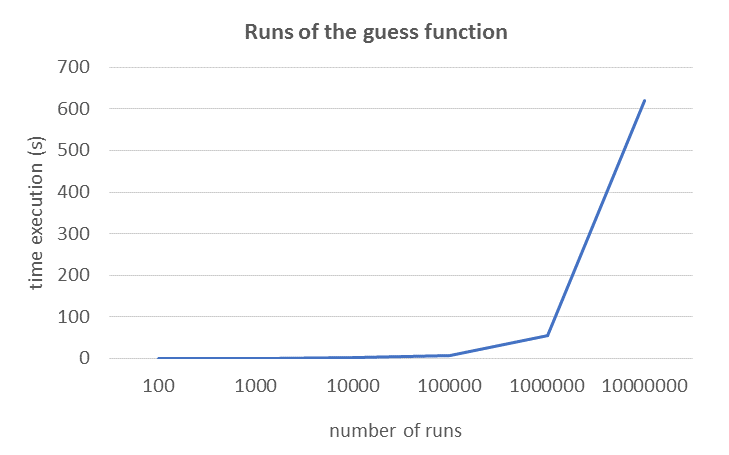
\includegraphics[width=3in]{figs/graph.png}}
		 	\vskip 8pt
		 	\defig{compl}{time execution of the function Guess}
		 \end{figure}

 
 \section{Next step}
 \begin{itemize}
	\item   I have to determine the maximum number of preferences models to have a believable time execution during the dialogue.
	\item Test the agent with the ToM execution.
	\item Profile the code in order to improve the time execution.
 \end{itemize}
 
 I've also made some changes to improve the existing code. 

%\section{Introduction}
%Theory of mind (ToM) is critical for success in social interaction. 
%social agents need ToM to successfully interact with humans.
%Principal challenge with ToM is insincerity  about user preferences and user goal.
%
%\section{Background ToM:}
%Modular theory, 
%simulation theory, 
%theory-theory, 
%and executive function theory.
%
%\section{Model of ToM}

\
\end{document}
